\chapter{Background}\label{ch:background}

seL4 is a formally verified and the fastest microkernel in the world with lots of awesome features (\cite{Klein_EHACDEEKNSTW_09}). The componentized system architecture that seL4 implements enforce the isolation between those untrusted components and other trusted components running on top of the kernel. seL4 was born for safety. The fine-grained capability-based access control model carefully manages the access to the hardware resources from the software components. 

The secure and well design of the seL4 microkernel together with the formal verification ensure the kernel itself is robust and is the ideal foundation to build a secure system on top of it (\cite{Klein_AEHCDEEKNSTW_10}). What's more, seL4 is not only secure but also fast. With its performant IPC mechanisms and most advanced mixed critical real-time systems (\cite{Lyons_Heiser_14}), the seL4 is capable to handle a wide range of real-world scenarios. However, seL4 is relatively young comparing to other mainstream kernels, such as Linux. And its ecosystem is in growing. For those seL4 developers, there are limited tools that can be used while developing seL4 systems. However, Linux provides us a powerful developing environment with lots of useful tools. Therefore, the main motivation of this project is to explore some ways to leverage the Linux features in terms of development to make developing seL4 systems much easier and faster.

\section{Challenge}

Developing applications targeted for seL4 in Linux is challenging because seL4 as a microkernel has different semantics and OS model based on seL4 comparing with Linux (In figure \ref{fig:osmodel}).

\begin{figure}[h]
    \copyrightbox[b]{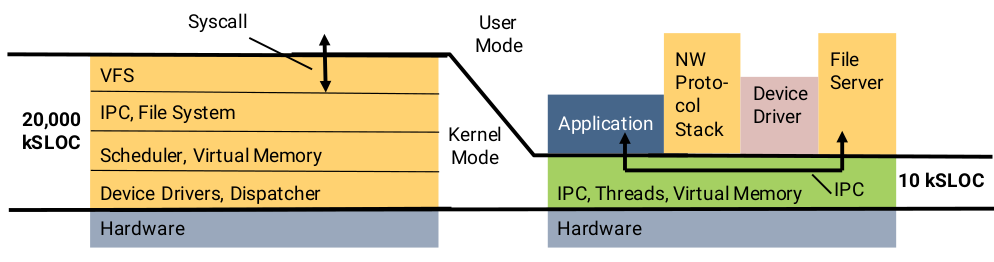
\includegraphics[width=0.9\textwidth, height=0.5\textwidth]{ch2/OS models.png}} % 
    {Source: "The seL4 Microkernel – An Introduction" (p. 3), by Gernot Heiser, 2020, the seL4 foundation. Copyright  under the Creative Commons Attribution-ShareAlike 4.0 International (CC BY-SA 4.0) License.}
    
    \caption{Linux based OS model vs seL4 based OS model.}
    % {\tiny Note: The picture comparison between monolithic OS vs microkernel OS model. Reprinted from "The seL4 Microkernel – An Introduction" (p. 3), by Gernot Heiser, 2020, the seL4 foundation. Copyright  under the Creative Commons Attribution-ShareAlike 4.0 International (CC BY-SA 4.0) License.}
    \label{fig:osmodel}
\end{figure}

Linux as a monolithic kernel, the kernel itself provides a wide range of OS services. The drivers, OS components are implemented inside of the kernel. All those OS services execute in kernel mode. While in seL4, to guarantee the strong isolation of different OS components, seL4 itself is just a thin wrapper of the underlying hardware providing minimal critical services of the hardware resources. And the OS services are implemented at the user level as separate components. Such design minimizes the TCB(Trusted Computing Base). 

In a monolithic kernel, the user-level applications request the OS services through the system call interfaces that are exported to the user level. A system call will cause a context switch from the user mode to the kernel mode. And the kernel will serve the OS requests by itself. For example, an I/O request from the user level will trigger the system call and the kernel will dispatch such request to the corresponding handler. In Linux, this might be a handler in the VFS layer. Then the VFS layer handler will find the particular File system handler and finally, it will invoke the driver to perform the I/O. After the system call getting triggered, everything happens in the kernel mode until the requests have been served. However, in the seL4 based OS model, it works differently. First, to clarify the term, we are going to call anything that runs in seL4 user space the seL4 applications. Also, we distinguish those applications into client applications that request OS  services and those server applications that serve the OS services. And the rest of the article, we will use the seL4 application as the term to make the description easier. When the seL4 client applications request OS services, it will invoke IPC mechanisms provided by the seL4 kernel. The seL4 IPC is a protected remote procedure call that can invoke the function in another seL4 application, which usually is the seL4 server applications securely. The IPC message passing is the main system call in the seL4, it triggers the context switch to the kernel mode, and the sel4 microkernel will then transport the input to the authorized seL4 server application via an exported entry point. Those requests are served by the seL4 serve application at the user level.
The seL4 client applications and seL4 server applications are isolated components, which ensures the security of the whole system.

Since, the main problem here is that seL4 and Linux have different semantics and program flow of serving OS services, the final goal of this project will be providing methods for developing seL4 user-level systems which can either run on Linux or seL4. In other words, we need to provide compatibility between seL4 applications and Linux.

\section{Related Work}

\subsection{QEMU}

% QEMU, a Fast and Portable Dynamic Translato

One way to achieve compatibility is to leverage hardware emulation or virtualization technology (\cite{enwikiqemu}). QEMU provides us both. It's a machine emulator supporting a wide range of ISA as well as a virtualizer providing us the hardware virtualization feature if the guest's ISA is the same as the host's ISA. With those features, we are capable of running the seL4 microkernel on top of the Linux. And from the seL4 user-level applications' view, they are still running on top of the seL4 microkernel. And the QEMU provides the compatibility between the seL4 microkernel and the underlying Linux kernel. 

QEMU uses portable dynamic translation to emulate the full system including processors and peripherals. By leveraging the advantages of hardware extensions such as Intel VT-X, QEMU can be used with KVM to run a virtualized guest OS in near-native speed. Moreover, the QEMU uses a dynamic binary translation approach, which means it's binary compatible. The way it works is QEMU will convert the guest instruction set into the host instruction set, then it will split instructions into fewer simpler instructions and use the dynamic code generator to assemble instructions into functions.

Although QEMU is an efficient dynamic translator (\cite{QEMU}), which makes QEMU significantly faster than other emulators, the overhead of doing that can't be ignored. On the other hand, QEMU provides its debugging interfaces which can be used to debug the guest system. However, the design goal of QEMU focuses on low-level machine emulation. It can be useful for inspecting each instruction's execution of the CPU, but it's difficult to use from a high-level seL4 developers' perspective. Because the debugger is not OS aware, the guest OS's context switch might confuse the debugger.

\subsection{Cygwin}

% Cygwin32: A Free Win32 Porting Layer for UNIX Applications

The Cygwin is a compatibility layer that allows UNIX-like applications to run on top of Windows (\cite{enwikicygwin}). This is achieved by introducing a DLL called cygwin1.dll which acts as an emulation layer providing substantial POSIX system call functionalities providing a Linux look and feel. While Cygwin uses newlibc as its C library. With Cygwin, users can access several standard UNIX utilities such as bash, etc.

Cygwin began development in 1995 at Cygnus Solutions. In the project, developers provided interfaces called Cygwin API to add the missing UNIX-like functionalities in Win32 API, such as fork, signals, select, etc (\cite{Cygwin}). Cygwin will not magically make any UNIX-like application's binary code runnable on top  Windows directly. To make it work, the source code of the application is required. The source code can be compiled under the Cygwin and linked with the shared library which implements the POSIX system call semantics using the Win32 APIs and native NT APIs. After executing the application, the Cygwin DLL will be loaded into the application's test region so that it has full access to the whole process. Next, shared memory is created containing the instances of the resources that the shared library can access. Therefore, the OS resources such as file descriptors can be tracked. Besides such shared memory regions, each process also has its resource bookkeeping structures, such as signal masks, PID, etc.

Cygwin has several nice designs to implement the POSIX features in Windows. For example, it handles signals by starting a separate thread from the library for only signal handling purposes. This thread waits for the Windows event used to pass signals to the process, and scan through its signal bitmask to handle the signals appropriately. While since such thread resides in the same address space as the executing program, the signal sending function for sending a signal to other processes is wrapped with a mutex, and the signal sending function which sends the signal to itself is wrapped by separate semaphore or event pair to avoid them being interrupted. 

Another example is the implementation of sockets. It's mapped on top of the Winsock which is implemented as Berkeley sockets by Microsoft with lots of modification. Since UNIX domain socket is not provided in Windows, Cygwin implements it with the local IPv4 as the address family. Besides, Cygwin provides the Winsock initialization on the fly, as the Winsock requires to be initialized before the socket function is called. For implementing the POSIX select, Cygwin implements the polling of file handles besides socket type handles by sorting the file descriptors into different types and creating a thread for each type of the file descriptors present to poll those file descriptors with Win32 API. Such a design is because the Winsock only works on socket type file descriptors.              
Although Cygwin implements lots of POSIX features, not all of them mapped well into Windows due to the huge difference in terms of semantics and underlying design between UNIX-like OS and Windows. For example, in UNIX-like systems, the $fork()$ system call provides a way to create a child process that copies the parent's address space. While there are no appropriate process creation functions in Windows which can be mapped on top of it. 

On the other hand, implementing $fork()$ semantics in Windows requiring to copy all of the executable binary and all the DLLs loaded statically or dynamically to be identical as to when the parent process has started or loaded a DLL. This can be problematic as Windows allows the binaries to be renamed to even removed to the recycle bin while the binary is executing, which means they can reside in a different directory or have a different file name. While to allow an executing process to fork requires access to the binary file via their original filenames. The solution to this problem is that Cygwin will try to create a private directory that contains the hardlink to the original files and remove it when no process is using it. When the parent process wants to fork a child process, it will first initialize a space in Cygwin process table for the child and create a suspended child process using Win32 CreateProcess system call. 

After that, the parent process will use setjump to save the context and set a pointer to the current context in the Cygwin shared memory, and fill the child process's .data and .bss section with its own address space. Next, the parent process will block on a mutex and the child process will run and use the longjump to jump to the saved jump buffer. Then child process will release the mutex that the parent is blocked on and waits for another mutex. The parent process will copy its stack and heap into the child process space then release the mutex that the child is blocking on and return from the fork call. Finally, the child process will wake up and recreates any memory-mapped areas that passed to it and return from the fork call. However, such implementation is not perfectly reliable as in Windows, Windows implements the ASLR starting from Vista, which means the stack, heap, text, and other regions may be placed in different places in each process. This behavior interferes with the POSIX fork's semantic that is the child process has the same address space as the parent process. In that case, Cygwin will try to compensate the movable memory regions at the wrong place but can't do anything with those unmovable regions such as the memory heap.

In summary, adding compatibility at the API layer can solve most of the problems when attempting to run applications from foreign systems. While the downside is that, apparently this will only work when the user of Cygwin can obtain the source code of the application. Meanwhile, it's very difficult to implement every POSIX system call in Windows correctly due to the huge difference between the internal design and the semantics. 

Even though Cygwin is used to make UNIX-like applications compatible with the Windows environment, we can still leverage the nice idea that Cygwin uses. To emulate seL4 in Linux we can link applications to a specific library that remaps the system calls with the underlying host's system calls.

\subsection{Wine}

% https://en.wikipedia.org/wiki/Wine_(software)#Basic_architecture

As mentioned before Cygwin is an API-compatible solution for providing compatibility between Windows and Linux. The next related project we are going to introduce is called Wine which is ABI compatible. Wine is a project that provides the compatibility layer to run Windows applications in UNIX-like operating systems (\cite{enwikiWine}). However, Wine doesn't emulate the internal Windows logic like a virtual machine or an emulator. Instead, it directly translates the Windows ABI into POSIX-compliant calls. Besides, Wine also provides various Windows services through Wineserver as well as other Windows components. In Wine's architecture, it implements Windows's ABI entirely in the user space, rather than a kernel module. 

A system call from a Windows application usually invokes a particular DLL library, which in turn invokes the user-mode GDI/user32 libraries, and then finally invokes the system calls via Win32 subsystem. However, since the architecture of Windows OS is a hybrid model of monolithic kernel combined with the microkernel, some OS services run as separate processes, so applications need to invoke RPCs to communicate the user-mode services. In that case, this is somehow similar to how seL4 applications request OS services. Although Wine implements the Wineserver to provide services that are provided by the Windows kernel, as well as other OS functionalities, it's impossible to implement all the aspects of the Windows kernel as well as to use native Windows drivers due to the internal architecture of Wine. 

With a similar idea as the Wine project, we can target the emulation layer of seL4 applications at the kernel ABI layer to achieve the binary compatibility as Wine does.       

\subsection{User-mode Linux}

UML is an old project used to port a Linux kernel to the userspace. This can be helpful to the system developers as it provides a nice way to develop and debug the kernel as well as to make several interesting applications possible for Linux (\cite{JD06}). 

In UML's architecture, it treats Linux as a platform to which the kernel can be ported. All the implementation fully leverages the Linux system calls without any modification of the host kernel. And all the user-level code can run natively on the processors without any instruction emulation overhead. The implementation creates a separate thread that uses the $ptrace()$ system call to trace all the other threads running in UML. 

\subsubsection{System Call}

Since the transition between user mode and the kernel mode is controlled by the tracing thread, it will intercept all the signals and system calls that the running process issues and then transit from the user mode to the kernel mode and continue executing the particular process without tracing it. The distinguishment of the user mode and the kernel mode is whether the process is being traced by the tracing thread. After changing the register which contains the syscall number into the syscall number for $getpid()$ and restoring a previously saved thread registers state, the tracing thread will invoke the syscall handler to accomplish the syscall request, then finally return the process to the user mode. 

\subsubsection{Trap and Fault}

UML not only virtualizes system calls but also implements several other Linux OS services and functionalities. For example, to handle the processor traps or faults, it implements those with signals and installs handlers for each. Once the tracing thread captures the signals that the process received, it will switch to the kernel mode and continue executing the process in the handler.

For the memory fault, UML implements with the $SIGSEGV$ and invokes the handler to figure out whether the fault was because of legal access to an unmapped page or illegal memory access. 

\subsubsection{Interrupt}

UML also implements external interrupts and timer interrupts using $SIGIO$ and $SIGALARM$ or $SIGVTALARM$ depending on whether the interrupted process is idling or not. For the external interrupts, it uses $select$ to check which file descriptor has received input then invokes the IRQ handler. For the timer interrupt, UML also treats it similarly to treating the external interrupt and invokes the particular IRQ handler. 

\subsubsection{Scheduling}

For process scheduling, UML implements scheduling processes by stooping an outgoing one and running an ingoing one as each process has its thread belongs to it. Since each process has its own address space, UML also manages the page mapping of each process as well as the $SIGIO$ queued in each process.

\subsubsection{Virtual memory}

In UML, the kernel and process's virtual memory is implemented as a physical memory-sized file mapping into their address spaces. However, some regions in the address space will be reserved by placing kernel code and data which is unusable.

\subsubsection{Host filesystem access}

UML also implements a virtual file system called $hostfs$ which translates the directly into the functions in the host's $libc$. Hence, it provides direct access to the host filesystem.

UML was a nice project showing a novel way to use Linux interfaces to implement itself, also it demonstrated that porting a kernel in the userspace can be beneficial to both kernel and application development.

From this project's perspective, UML gives us the hint of how to leverage $ptrace$ to intercept the system call from the process being traced as well as how to simulate the kernel in the userspace.




